\documentclass[a4paper]{article}

\usepackage[czech]{babel} %https://github.com/michal-h21/biblatex-iso690
\usepackage[
   backend=biber      % if we want unicode 
  ,style=iso-numeric % or iso-numeric for numeric citation method          
  ,babel=other        % to support multiple languages in bibliography
  ,sortlocale=cs_CZ   % locale of main language, it is for sorting
  ,bibencoding=UTF8   % this is necessary only if bibliography file is in different encoding than main document
]{biblatex}

\usepackage[utf8]{inputenc}
\usepackage{fancyhdr}
\usepackage{amsmath}
\usepackage{amssymb}
\usepackage[left=2cm,right=2cm,top=2.5cm,bottom=2.5cm]{geometry}
\usepackage{graphicx}
\usepackage{pdfpages}
\usepackage[version=4]{mhchem}
\usepackage{url}

\usepackage{siunitx}
\sisetup{locale = DE, separate-uncertainty = true} %    kdybych chtel +/-

\usepackage{float}
\newfloat{graph}{htbp}{grp}
\floatname{graph}{Graf}
\newfloat{tabulka}{htbp}{tbl}
\floatname{tabulka}{Tabulka}

\renewcommand{\thefootnote}{\roman{footnote}}

\pagestyle{fancy}
\lhead{Praktikum II - (26) Elektrická vodivost elektrolytů}
\rhead{Vladislav Wohlrath}
\author{Vladislav Wohlrath}

\bibliography{source}

\begin{document}

\begin{titlepage}
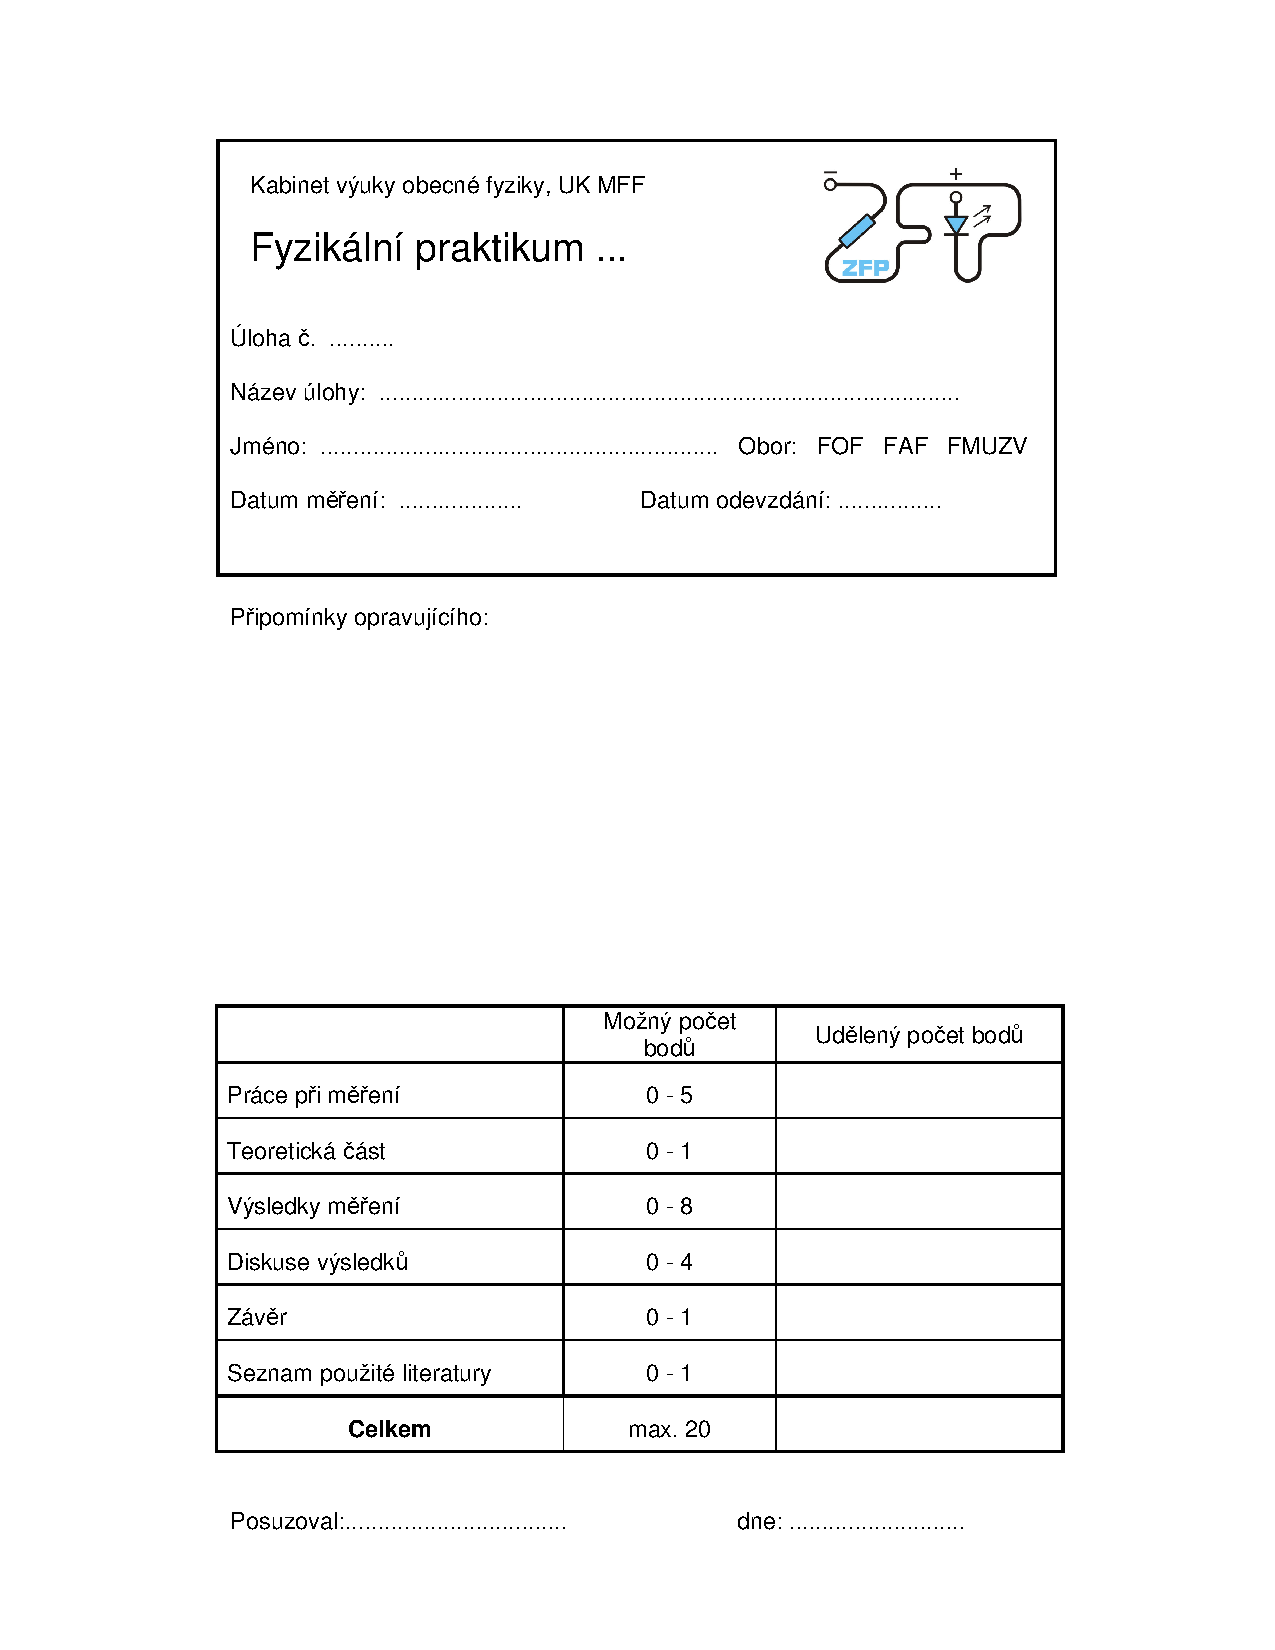
\includepdf[pages={1}]{./graficos/titlelist.pdf}
\end{titlepage}

\section*{Pracovní úkoly}
\begin{enumerate}
\item Změřte měrnou elektrickou vodivost (konduktivitu) destilované vody.
\item Do odměrných baněk \SI{100}{\milli\litre} napipetujte postupně 1, 2, 4, 6, 8 a \SI{10}{\milli\litre} slabého a silného elektrolytu a doplňte baňky do \SI{100}{\milli\litre} (spodní meniskus hladiny se musí krýt s ryskou).
\item Změřte konduktivitu připravených vzorků.
\item Stanovte molární konduktivitu těchto vzorků a znázorněte ji graficky jako funkci $\sqrt{c}$.
\item Diskutujte rozdíly mezi koncentrační závislostí molární konduktivity slabého a silného elektrolytu.
\item Lineární extrapolací pro nekonečné zředění (nulovou koncentraci) stanovte $\Lambda_0$.
\item Kalibraci elektrody pomocí roztoku KCl neprovádějte.
\end{enumerate}

%Teoretická část
\section*{Teoretická část}
Podle stupně disociace dělíme elektrolyty na silné (stupeň disociace blízký jedné) a slabé (velmi nízký stupeň disociace).

Měříme závislost měrné voivosti $\sigma$ roztoku na molární koncentraci $c_M$.
Definujeme molární konduktivitu \cite{skripta}
\begin{equation}
\Lambda = \frac{\sigma}{c_M} \,.
\end{equation}

Molární konduktivita se mění s koncentrací, neboť je na ní závislá pohyblivost iontů.
Pro silné a slabé elektrolyty je koncentrační závislost různá.
U silných elektrolytů lze závislost popsat empirickým vztahem \cite{skripta}
\begin{equation} \label{e:silne}
\Lambda = \Lambda_0 - k \cdot \sqrt{c_M} \,,
\end{equation}
kde $k$ je konstanta a $\Lambda_0$ je limitní molární konduktivita při nekonečném zředění.

%Výsledky měření
\section*{Výsledky měření}

%Diskuze výsledků
\section*{Diskuze}

Z grafu \ref{g:sCl} vyplývá, že závislost konduktivity \ce{HCl} na koncentraci je velmi dobře lineární a z grafu \ref{g:lCl} nevyplývá žádná jednoduchá závislost molární konduktivity na koncentraci.
Závislost není dokonce ani monotónní, což neodpovídá empirickému vzorci \eqref{e:silne}.
První čtyři hodnoty naznačují klesající trend, pokud bychom proložili přímkou jen je (v grafu přerušovanou čarou), obdrželi bychom mírně odlišnou hodnotu $\Lambda_0=\SI{38.4(2)}{\milli\siemens\metre\squared\per\mole}$. Tento postup ale považujeme za neoprávněný.
Konstanta $k$ je pravděpodobně příliš malá na to, abychom ji změřili našimi prostředky.

\ce{CH_3COOH} není silný elektrolyt a proto pro ni neplatí \eqref{e:silne}. Z grafu \ref{g:lCH} je vidět, že závislost $\Lambda(\sqrt{c_M})$ v měřeném rozsahu určitě není lineární.
Pokud bychom předpokládali, že se na intervalu $\left(0;\num{0.7}\right)$ chová lineárně, extrapolací bychom získali $\Lambda_0=\SI{17.8(5)}{\milli\siemens\metre\squared\per\mole}$. Odpovídající závislost $\sigma(c_M)$ je zakreslena do grafu \ref{g:sCH}. Ve skutečnosti ale graf \ref{g:lCH} naznačuje spíše ryze konvexní průběh, takže můžeme usuzovat, že skutečná hodnota je vyšší.
Uvedené úvahy jsou ovšem pouhé dohady, pro spolehlivé určení $\Lambda_0$ pro \ce{CH_3COOH} by bylo nutné důkladnější měření a studium slabých elektrolytů.


Zjistili jsme, že molární konduktivita silného elektrolytu je přibližně čtyřikrát vyšší než slabého elektrolytu.
Se zvyšující se koncentrací u slabého elektrolytu velmi rychle klesá, zatímco u silného elektrolytu klesá velmi pomalu, či je dokonce konstantní.

%Závěr
\section*{Závěr}


\printbibliography[title={Seznam použité literatury}]

\end{document}